\normalfalse \difficiletrue \tdifficilefalse
\correctiontrue

%\UPSTIidClasse{11} % 11 sup, 12 spé
%\newcommand{\UPSTIidClasse}{12}

\exer{Barrière Sympact $\star\star$ \label{CIN:02:B2:13:14}}
\setcounter{question}{0}
\marginnote{\xpComp{CIN}{02}}
%\UPSTIcompetence{B2-13}
\index{Compétence B2-13}\index{Compétence CIN-02}
\index{Barrière Sympact}
\ifcorrection
\else
\marginnote{\textbf{Pas de corrigé pour cet exercice.}}
\fi

\ifprof
\else
Soit le mécanisme suivant. On a $\vect{AC}=H\vect{j_0}$, $\vect{CB}=R\vect{i_1}$ et $\vect{AB}=\lambda(t) \vi{2}$. De plus, 
$H=\SI{120}{mm}$ et $R=\SI{40}{mm}$. 

\begin{marginfigure}
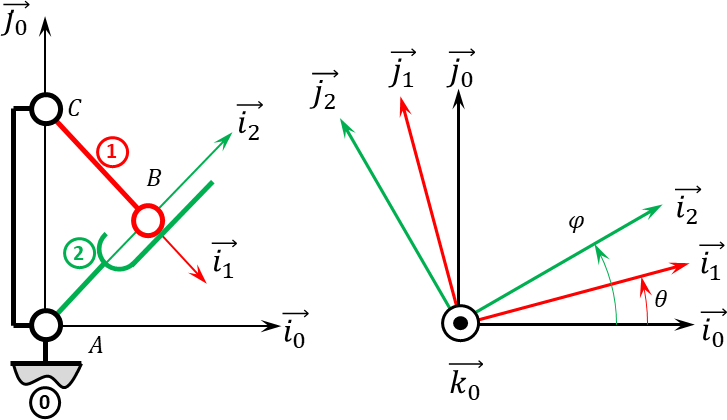
\includegraphics[width=\linewidth]{14_01}
\end{marginfigure}
\fi


\question{Calculer $\vectv{B}{1}{0}$ ?}
\ifprof
$\babarv{B}{C}{1}{0}$ 
$=\vect{0}-R\vi{1}\wedge\thetap\vk{0}$
$=R\thetap\vj{1}$.

(Possibilité d'utiliser la dérivation vectorielle.)

\else
\fi

\question{Calculer $\vectv{B}{2}{0}$ ?}
\ifprof
$\babarv{B}{A}{2}{0}$ 
$=\vect{0}-\lambda \vi{2}\wedge\varphip\vk{0}$
$=\lambda\varphip\vj{2}$.

(\textbf{Impossibilité} d'utiliser la dérivation vectorielle.)

\else
\fi

\question{Justifier que $\vectv{B}{2}{1}\cdot\vect{j_2}={0}$.}
\ifprof
La liaison entre \textbf{2} et \textbf{1} est une liaison ponctuelle de normale $\vj{2}$. Il n'y a donc pas de vitesse sur cette direction (ce qui de plus provoquerait une rupture de contact en $B$). 
\else
\fi

\question{En déduire une relation cinématique entre les différentes grandeurs.}
\ifprof
En utilisant la décomposition du vecteur vitesse, on a
$\vectv{B}{2}{1}\cdot \vj{2} =\left( \vectv{B}{2}{0} - \vectv{B}{1}{0}\right) \cdot \vj{2}$
$ \Leftrightarrow {0} =\left( \lambda\varphip\vj{2} - R\thetap\vj{1}\right) \cdot \vj{2}$
$ \Leftrightarrow {0} = \lambda\varphip - R\thetap \cos \left( \varphi - \theta\right)$

\else
\fi


%\question{En déduire la course de la pièce \textbf{3}.}
%\ifprof
%\else
%\fi



\ifprof
\else
\footnotesize
\ifcolle
\else
\begin{marginfigure}
\begin{tabular}{|p{.9\linewidth}|}
\hline
Indications :
\begin{enumerate}
\item $\vectv{B}{1}{0}=R\thetap\vj{1}$.
\item $\vectv{B}{2}{0}=\lambda\varphip\vj{2}$.
\item .
\item $ \lambda\varphip - R\thetap \cos \left( \varphi - \theta\right)=0$.
\end{enumerate} \\ \hline
\end{tabular}
\end{marginfigure}
\fi
\normalsize

\begin{flushright}
\footnotesize{Corrigé  voir \ref{CIN:02:B2:13:14}.}
\end{flushright}%
\fi